\newpage
\section{WegGL \& Shaders}
 %\begin{figure}[H]
 %\centering
 %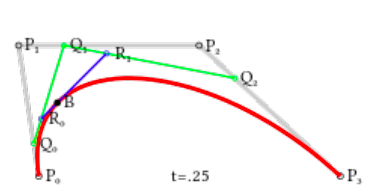
\includegraphics[width=.5\linewidth]{bezier} 
 %\end{figure}
\subsection{Intro}
The \textbf{OpenGL API} is a software interface for graphics hardware. A program can use OpenGL API for calling some prepackaged functionality to:
\begin{itemize}
\item \textbf{Define models}
\item \textbf{Use Textures}
\item \textbf{Perform operations (e.g. projections}
\end{itemize}
in order to \textbf{render images} (usually 3D).\\
The OpenGL specification is implemented as the \textbf{OpenGL library} by hardware vendors ( NVIDIA,AMD...) making OpenGL \textbf{portable}. It can also be implemented\textbf{without GPU}.
\\OpenGL is implemented as \textbf{client-server} system : 
\begin{itemize}
\item \textbf{Client side}: the application code in the main CPU memory  (issues commands) 
\item \textbf{Sever side} :hardware and memory on the graphics card (executes the commands to produce the final image)
\end{itemize}
To keep track of all the \textbf{state-variables} OpenGL uses a \textbf{state model} . This avoids \textbf{passing to many arguments} in function calls and allows to \textbf{keep the state value} until it is changed by some other function.\\
\subsection{GLSL}
Up to 2004 as graphics adapters evolved OpenGL was improved by adding \textbf{new functionalities}. However the many new technological improvements made issuing \textbf{fixed procedures} very expensive so the \textbf{OpenGL Shading Language (GLSL)} , a C-like language , was introduced to specify \textbf{rendering operations} only.\\
With GLSL new \textbf{derivative APIs} were introduced : 
\begin{itemize}
\item \textbf{OpenGL ES} for \textbf{embedded systems} with limited system resources.
\item \textbf{WebGL} , an OpenGL-style rendering within \textbf{web-browsers} using \textbf{Java Script} to access the\textbf{ OpenGL ES 2.0} functionalities and the \textbf{HTML Canvas elements} for drawing.
\end{itemize}

\subsection{WebGL - Client}
\subsubsection{Canvas}
WebGL takes advantage of the \textbf{Canvas element} of HTML5:
\begin{itemize}
\item allows \textbf{scriptable rendering} of graphics within the browser
\item provides the default \textbf{FrameBuffer}, a region of \textbf{physical memory} in the GPU used to temporarily store an image for rendering.
\item supports different API (like WebGL...)
\item has \textbf{width,height,ID} attributes
\item the area within the canvas can be modified with \textbf{JavaScript}
\end{itemize}
 \begin{figure}[H]
 \centering
 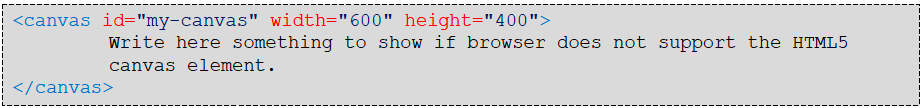
\includegraphics[width=.6\linewidth]{canvas} 
 \end{figure}

 
\subsubsection{Context}
The first element a program must create to draw graphics is the \textbf{Context}. It provides \textbf{internal data structure} for keeping track of the state settings and operations. Examples of state-values are \textit{current path, current fill and stroke, line width and pattern, alpha transparency, antialiasing ,blend mode , shadows,transformation matrix, text attributes}.\\
It can be requested using \texttt{.getContext(contextID, *args...)} JavaScript function on the \textbf{canvas element}. The \texttt{contextID} argument can have values :
\begin{itemize}
\item \texttt{2D}
\item \texttt{webgl/experimental-webgl}
\end{itemize}
 \begin{figure}[H]
 \centering
 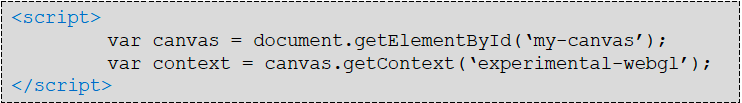
\includegraphics[width=.6\linewidth]{context} 
 \end{figure}

\subsubsection{Drawing with 2D Context}
Once the \textbf{frameBuffer} (provided by the \texttt{Canvas} element) and the \textbf{context} are provided , drawing can begin. To start drawing the data for \textbf{constructing the shapes} must be specified through \textbf{geometric primitives}. \textbf{HTML 2d context} makes available :
\begin{itemize}
\item \textbf{Rectangles}
\begin{itemize}
\item \texttt{context.rect(x,y,width,height} $\to$ creates an \textbf{invisible} rectangle object to be further defined by commands such as \texttt{.stroke()} or \texttt{.fill()}
\item \texttt{context.fillRect(x,y,width,height)} $\to$ create a filled rectangle with no border line
\item \texttt{context.stroke(x,y,width,height)} $\to$ creates an empty rectangle with border line

\end{itemize}
\item \textbf{Paths (lines or circles)}
\begin{itemize}
\item \texttt{context.beginPath()} $\to$ begins a path or resets the current one
\item \texttt{context.moveTo(x,y)} $\to$ moves the path to the specified point on the canvas, \textbf{without creating a line}
\item \texttt{context.lineTo(x,y)} $\to$ adds a new point and \textbf{creates a line} from that point to the last specified one
\item \texttt{context.closePath()} $\to$ creates a path from the current point back to the starting point
\item \texttt{context.arc(x,y,r,sAngle,eAngle,counterclockwise)} $\to$ creates an arc/curve 
\item \texttt{context.arcTo(x1,y1,x2,y2,r)} $\to$ creates an arc/curve between two tangents.
\end{itemize}
\end{itemize}
The 2D context has a \textbf{coordinate system} similar to the one of the screen, with values also expressed in pixels. The coordinates in the canvas are transparently mapped on-screen by the context.
  \begin{figure}[H]
 \centering
 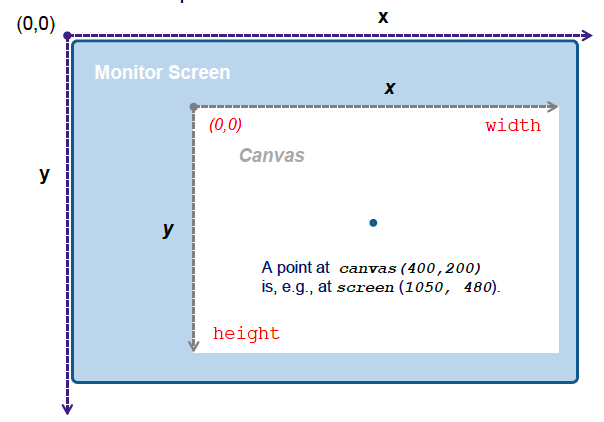
\includegraphics[width=.5\linewidth]{canvas2} 
 \end{figure}

\subsubsection{Drawing with webgl Context}
With respect to the \textbf{2D context} , the \textbf{experimental-webgl/webgl} context provides:
\begin{itemize}
\item A different \textbf{coordinate system}\\
Coordinates in webgl context start in the \textbf{middle of the canvas} with values expressed in \textbf{floating point numbers}. Its values for shapes can be \textbf{outside} the $[-1,1]$ range provided that some \textbf{computations} are made.
  \begin{figure}[H]
 \centering
 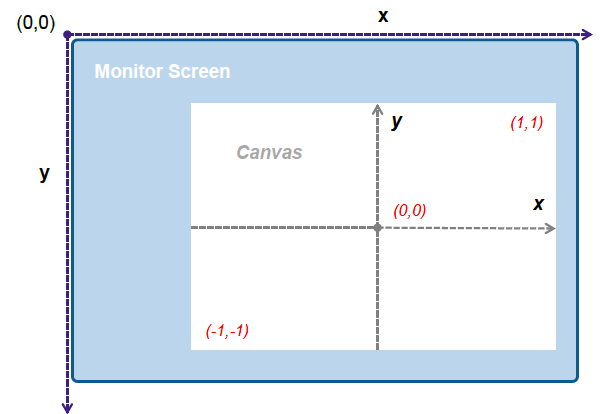
\includegraphics[width=.5\linewidth]{canvas3} 
 \end{figure}
 \item A different set of \textbf{geometric primitives}\\
 A webgl primitive is simply a \textbf{collection of vertices} hooked together in a predefined way. All primitives are 1d,2d or 3d ranging from simple lines to groups of triangles : all WebGL can do is visualize \textbf{points,lines and triangles} and apply \textbf{color and texture} to them. 
   \begin{figure}[H]
 \centering
 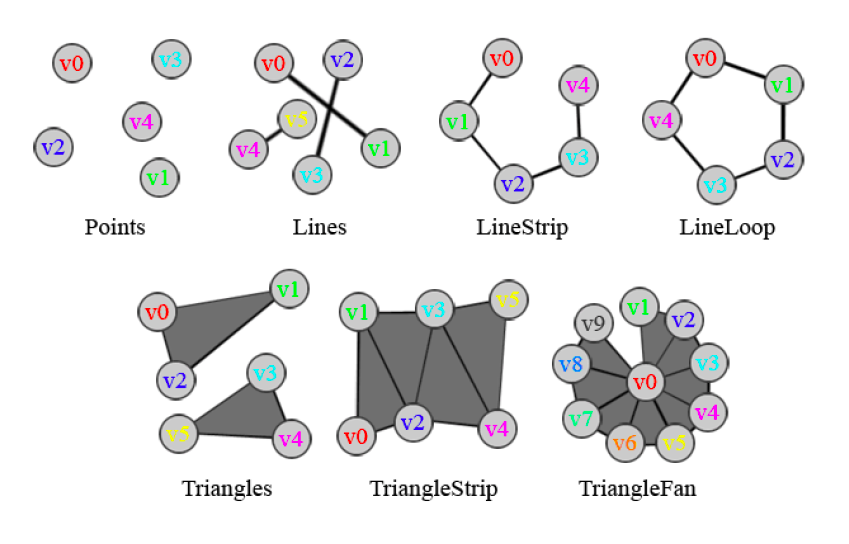
\includegraphics[width=.5\linewidth]{webglprimitives} 
 \end{figure}
\item A different set of \textbf{modes} for drawing\\
Unlike the 2d canvas context , the webgl context doesn't allow to directly set the color or location of a vertex into a scene. Furthermore shapes \textbf{cannot} be constructed using a list of fixed polygonal drawing functions (too many!). All data associated with vertices need to be streamed from JavaScript API to GPU and \textbf{only then} it will be possible to call the \textbf{draw} command. To pass vertex data, a \textbf{vertex buffer object VBO} ,which holds attributes such as \textbf{position,normals,texture,coordinates...} must be build :
\begin{enumerate}
\item Define an array holding the vertexes of the shape
   \begin{figure}[H]
 \centering
 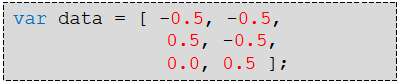
\includegraphics[width=.5\linewidth]{vbo1} 
 \end{figure}
\item Ask WebGL to reserve a \textbf{buffer}. Note that \texttt{gl} here corresponds to the variable returned by \texttt{canvas.getContext}
   \begin{figure}[H]
 \centering
 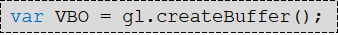
\includegraphics[width=.5\linewidth]{vbo2} 
 \end{figure}
 \item Set VBO buffer as active and bind to data type
    \begin{figure}[H]
 \centering
 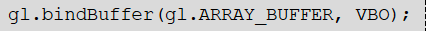
\includegraphics[width=.5\linewidth]{vbo3} 
 \end{figure}
 \item Place vertex data inside buffer. The \texttt{data} parameter should be casted to contain floats (required by JavaScript!) like : \texttt{new Float32Array(data) }
    \begin{figure}[H]
 \centering
 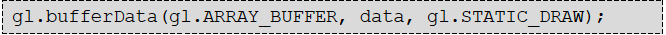
\includegraphics[width=.5\linewidth]{vbo4} 
 \end{figure}
\item  In webgl rendering operations must use \textbf{GLSL} , which creates a program \textbf{server-side} that defines who the GPU will handle data send to it.

 \item Retrieve the handle to the location of GPU where the GLSL program expects to find the input data. The \texttt{"VertexPosition"} is defined in the GLSL program 
     \begin{figure}[H]
 \centering
 
\includegraphics[width=.5\linewidth]{vbo5} 
 \end{figure}
 \item \textbf{Data are sent}. It activates communication that from client reach the servev input location specified by \texttt{vertexPositionHandle}
      \begin{figure}[H]
 \centering
 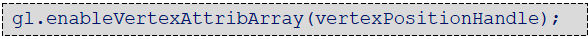
\includegraphics[width=.6\linewidth]{vbo6} 
 \end{figure}
 \item Let the GLSL program know how to interpret the data.\\
 \texttt{GLuint index} = handle to input location\\
 \texttt{GLint size} = how many values define the vertex\\
 \texttt{GLenum type} = the type of the data
 \texttt{GLboolean normalized} = if data requires normalization
      \begin{figure}[H]
 \centering
 
\includegraphics[width=.7\linewidth]{vbo7} 
 \end{figure}
 \item Draw by calling GLSL program \\
 First parameter is specifies the \textbf{primitive} to be used\\
 Second parameter is index of element to start drawing from \\
 Third parameter is number of vertexes
       \begin{figure}[H]
 \centering
 
\includegraphics[width=.5\linewidth]{vbo8} 
 \end{figure}
\end{enumerate}
\end{itemize}

Another important feature is \textbf{Aspect Ratio} : when setting up the canvas width and height might be different ( remember that pixels are usually \textbf{squared}). In this case the $[-1,1]$ coordinates are mapped \textbf{non-proportionally} to screen coordinates  : this results for example in a circle looking like an ellipse.\\
$$ \text{Aspect Ratio a} = \frac{\text{canvas.width}}{\text{canvas.height}}$$
So if the \textbf{y-coordinate} of a point is multiplied by the aspect ratio \textbf{or} the \textbf{x-coordinate} divided by it, the shape will result as intended.

\subsubsection{Drawing with webgl context : 3D}
When drawing a cube in WebGL different approaches can be used:
\begin{itemize}
\item \textbf{WireFrame Cube}\\
In this case only the edges are visible. Since the cube is composed of \textbf{8 vertices and 12 edges} the total number of vertices stores is \textbf{24} ( vertices are duplicated)
 \begin{figure}[H]
 \centering
 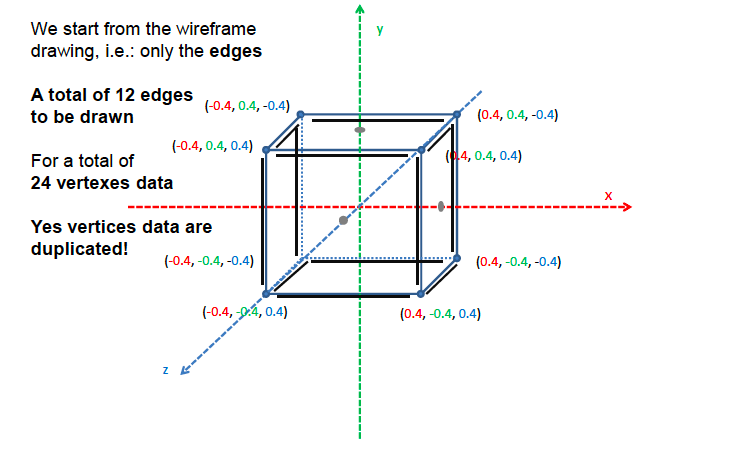
\includegraphics[width=.5\linewidth]{wireframe} 
 \end{figure}
The same procedure applies as for the 2D case applies. A difference is that since we're in 3D the \texttt{gl.vertexAttribPointer()} has as second parameter \textbf{3} instead of \textbf{2}.\\
The resulting figure will not appear as a cube since no \textbf{perspective} and no \textbf{view camera} have been implemented : these two can be stored in a \textbf{projection matrix} that is fed to a GLSL program (with some modifications to take the matrix into account). For the matrix you must get :
\begin{itemize}
\item \texttt{matrixPositionHandle = gl.getUniformLocation(program,'pMatrix')}
\item \texttt{gl.uniformMatrix4fv(matrixPositionHandle,gl.FALSE,\\ transposeMatrix(projectionMatrix)}
\end{itemize}
\item \textbf{Mesh cube}\\
In this case the cube is composed of a set of triangles. Each cube face has \textbf{2 triangles} for a total of \textbf{12 triangles}, each defined by 3 vertexes. So first define the \textbf{24 vertexes} than define a \textbf{index array} composed of 12x3 elements ( each row has 3 values indicating the vertex index making up the triangle)
 \begin{figure}[H]
 \centering
 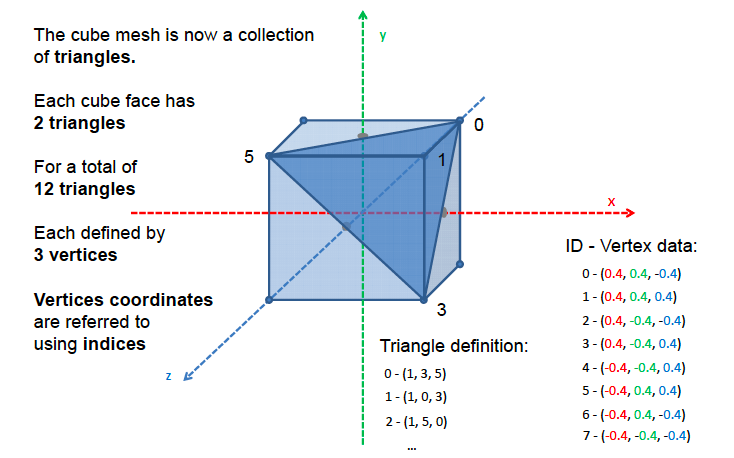
\includegraphics[width=.5\linewidth]{meshcube} 
 \end{figure}
  The index array needs its \textbf{own buffer} the  \textbf{IBO} buffer:
 \begin{itemize}
 \item \texttt{IBO = gl.createBuffer()}
 \item \texttt{gl.bindBuffer(gl.ELEMENT.ARRAY.BUFFER,IBO)}
 \item \texttt{gl.bufferData(gl.ELEMENT.ARRAY.BUFFER,new Uint16Array(indexes),\\gl.STATIC.DRAW)}
 \end{itemize}
 The draw function needs to be update : no longer \texttt{gl.drawArrays(gl.LINES,0,24}  but \texttt{gl.drawElements(gl.TRIANGLES, indices.length,gl.UNSIGNED.SHORT.INT,0 (starting point))}
\item \textbf{Mesh cube with colors}\\
In this case each vertex is composed of three positional argument + \textbf{3 RGB values}.
 \begin{figure}[H]
 \centering
 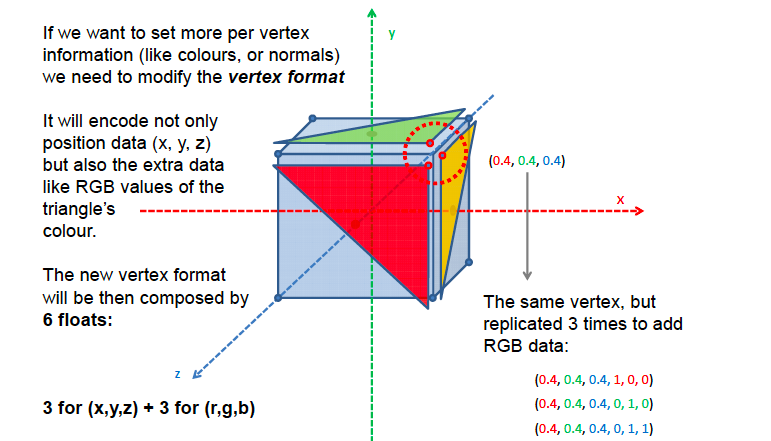
\includegraphics[width=.5\linewidth]{meshcubecolor} 
 \end{figure}
 An additional \texttt{vertexColorHandler} must be defined:
 \begin{itemize}
\item \texttt{vertexColorHandler = gl.getAttribLocation(program,'col1')}
\item \texttt{gl.enableVertexAttribArray(vertexColorHandler)}
\item \texttt{gl.vertexAttribPointer(vertexPositionHandler,3,gl.FLOAT,false,4*6 (4  bytes 6 values),4*3 (4 bytes staring skipping the first three positional args)}
 \end{itemize}
\end{itemize}

\subsection{GLSL - Server}
GLSL creates a program that defines how the GPU will handle the data sent to it. 
The rendering process follows a \textbf{Rendering Pipeline}:
 \begin{figure}[H]
 \centering
 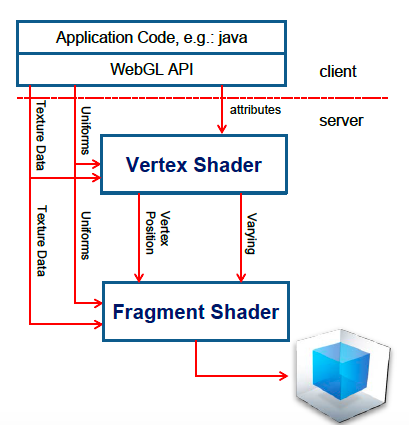
\includegraphics[width=.5\linewidth]{renderingpipe} 
 \end{figure}
\textbf{Shaders} are \textbf{individual programs} written in \textbf{GLSL} that execute on graphics hardware to process vertices and perform rasterization tasks.
The WebGL pipeline deals with two shaders :
\begin{itemize}
\item \textbf{Vertex Shader}
\item \textbf{Fragment Shader}
\end{itemize}

\subsubsection{Vertex Shader}
The VS contains source code of operations that are meant to be performed on each
vertex that is processed :
\begin{itemize}
\item \textbf{World-View-Projection} computation
\item \textbf{Vertex color} computation
\item \textbf{Light color} when using the \textbf{Goureaud} method
\item ...
\end{itemize}
The VS is executed for \textbf{each vertex} so three times to render a triangle.
The outputs of this step are:
\begin{itemize}
\item Vertices are assembled according to the \textbf{mode} argument of the drawing command
\item Clipping and Screen coordinates are computed
\item primitive is converted to a 2D image (\textbf{rasterization}). Each point of the image contains information as \textbf{color} and \textbf{depth}
\end{itemize}

\subsubsection{Fragment Shader}
The FS contains source code of operations that are meant to be performed on each \textbf{fragment} that results from \textbf{vertex shader rasterization}.
A \textbf{fragment} is one of the 2D image grid squares along with its parameters of depth and other data :
 \begin{figure}[H]
 \centering
 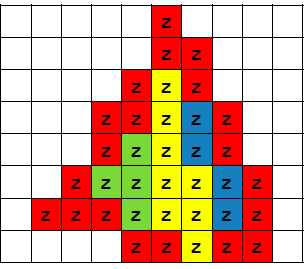
\includegraphics[width=.5\linewidth]{fragment} 
 \end{figure} 
Its operations are :
\begin{itemize}
\item \textbf{Anti-Aliasing} (can be done automatically)
\item \textbf{Depth-test} (can be done automatically)
\item \textbf{Color Blending} (can be done automatically)
\item \textbf{Dithering} (can be done automatically)
\item \textbf{Texturing} (must be done manually)
\item \textbf{Color and light computation in Phong mode} (must be done manually)
\end{itemize}
At the end of the pipeline the image is ready to be displayed.

\subsubsection{Data Types}
Data must be passed through the different steps in the pipeline.
There are different types: 
\begin{itemize}
\item \textbf{Attributes}\\
These are values that change per vertex ( for example x,y,z positions)
\begin{itemize}
\item (x,y,z) $\to$ 12 bytes
\item (x,y,z,r,g,b) $\to$ 24 bytes
\item (x,y,z,nx,ny,nz) $\to$ 24 bytes
\item (x,y,z,nx,ny,nz,u,v) $\to$ 32 bytes
\end{itemize}
\item \textbf{Uniforms}\\
These are per-program variables that are \textbf{constant} during execution.
Examples are \textbf{Transformations matrices}. Uniforms can be passed to \textbf{both} shaders.
\item \textbf{Texture data (Samplers)}\\
These are special uniform variables used for \textbf{texturing}.They are used to identify the texture object used for each \textbf{texture lookup}.	
\item \textbf{Varying}\\
Varying variables hold the result of VS execution that are used later in the pipeline (like partial results). These values are expected to be \textbf{interpolated} : this is because VS is executed only for each vertex but the FS is executed many more times (so must work on interpolated points)
\end{itemize}

\subsubsection{GLSL Program Language}
A GLSL shader program syntax is very C-like:
 \begin{figure}[H]
 \centering
 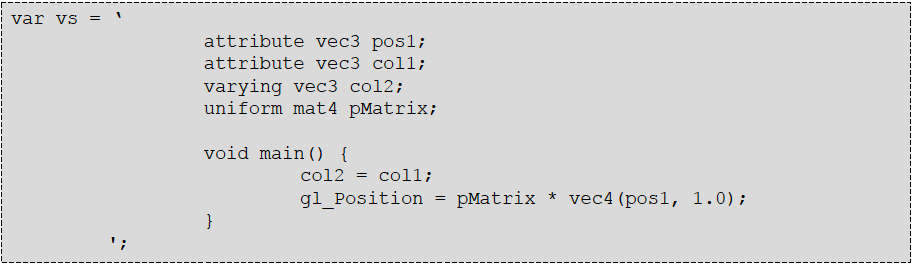
\includegraphics[width=.6\linewidth]{glsl} 
 \end{figure} 

The variable ,unlike C , are defined using \textbf{storage qualifiers,variable type and variable name}
 \begin{figure}[H]
 \centering
 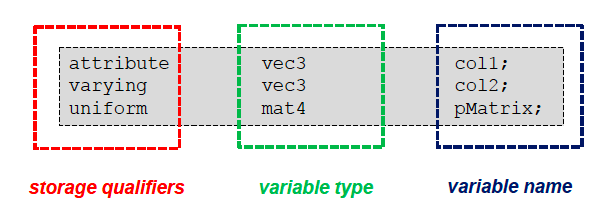
\includegraphics[width=.5\linewidth]{glslvars} 
 \end{figure} 
Accepted \textbf{storage qualifiers} are: 
\begin{itemize}
\item \texttt{const} $\to$ compile-time constant or read-only function parameter
\item  \texttt{attribute} $\to$ linkage between vertex shader and OpenGL ES for per-vertex data
\item  \texttt{uniform} $\to$ value does not change across the primitive being processed. They form the linkage between a shader,OpenGL ES and the application
\item  \texttt{varying} $\to$ linkage between VS and FS for interpolated data
\end{itemize}
Accepted basic \textbf{variable types} are:
\begin{itemize}
\item  \texttt{void} $\to$ no function return value or empty parameter list
\item  \texttt{bool}
\item  \texttt{int}
\item  \texttt{float}
\item  \texttt{vec2,vect3,vect4} $\to$ n-component floating point vector
\item  \texttt{bvec2,bvec3,bvec4} $\to$ boolean vector
\item  \texttt{ivec2,ivec3,ivec4} $\to$ signed integer vector
\item  \texttt{mat2,mat3,mat4} $\to$ 2x2,3x3,4x4 \textbf{float} matrix
\item  \texttt{sampler2D} $\to$ access a 2D structure
\item  \texttt{samplerCube} $\to$ access cubed mapped structure
\end{itemize}
\textbf{Vectors} are widely used. Here some characteristics:
\begin{figure}[H]
 \centering
 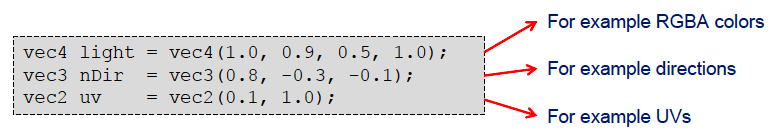
\includegraphics[width=.5\linewidth]{glslvecs} 
\end{figure} 
\begin{figure}[H]
 \centering
 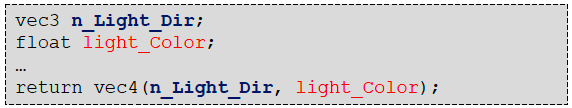
\includegraphics[width=.5\linewidth]{glslvecs2} 
\end{figure} 
\begin{figure}[H]
 \centering
 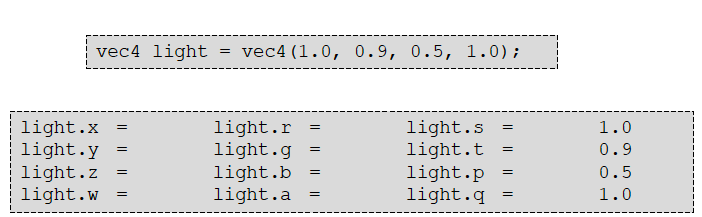
\includegraphics[width=.5\linewidth]{glslvecs3} 
\end{figure} 
\begin{figure}[H]
 \centering
 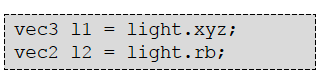
\includegraphics[width=.5\linewidth]{glslvecs4} 
\end{figure} 

GLSL provides also \textbf{functions} , which are similar to C:
\begin{figure}[H]
 \centering
 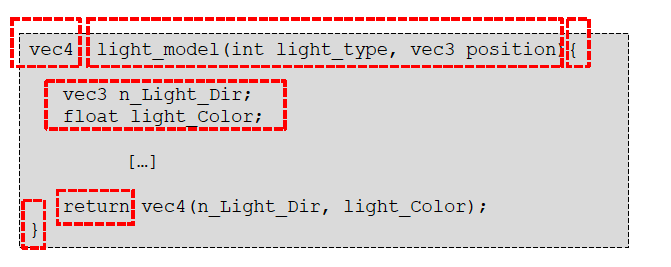
\includegraphics[width=.5\linewidth]{glslfuncs} 
\end{figure} 
The OpenGL provides \textbf{precision qualifiers} for \texttt{int}, \texttt{float} and \texttt{sampler} variables to \textbf{increase efficiency} and \textbf{decrease memory requirements} for shaders.
\begin{figure}[H]
 \centering
 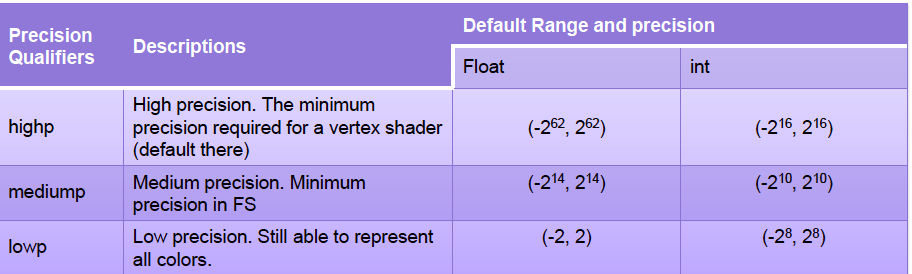
\includegraphics[width=.7\linewidth]{glslprecision} 
\end{figure} 
These precision qualifiers can be added:
\begin{itemize}
\item \textbf{before} the type specification \texttt{mediump vec3 col1}
\item \textbf{state for ALL variables} \texttt{precision mediump float}
\end{itemize}
There are also \textbf{Special Variables (global)} used to communicate with fixed function parts of the pipeline. They \textbf{do not} need to be declared but are \textbf{essential} :
\begin{itemize}
\item \texttt{gl-Position= pMatrix * vec4(pos1,1.0)} $\to$ for the VS which holds the \textbf{final} transformed vertex position in \textbf{screen-coordinates}
\item \texttt{gl-FragColor=vec4(col2,1)} $\to$ for the FS which holds the \textbf{final} fragment color in \textbf{RGBA}
\end{itemize}

\subsubsection{GLSL Compiling}
A shader must be \textbf{compiled} and \textbf{linked} before being used.
This is done by calling the proper functions \textbf{client-side}:
\begin{enumerate}
\item A shader object must be created for both \textbf{VS} and \textbf{FS} using the function \texttt{Object createShader(enum Type)} with the \textbf{handler} stored in a variable. The allowed \texttt{Types} are \textbf{Vertex-Shader} and \textbf{Fragment-Shader}
\item Shader must be loaded with a source string using \texttt{void shaderSource(Object shader, string source)}
\item Compile the shader by calling \texttt{void compileShader(Object shader)} (here a exception can occur!)
\item Create shader program object 	that contains the whole pipeline with \texttt{Object createProgram()} that returns a \textbf{pointer}.
\item Attach compiled shaders to the program with \texttt{void attachShader(Object program , Object shader)}
\item Link program using \texttt{void linkProgram (Object program)}
\end{enumerate}
\begin{figure}[H]
 \centering
 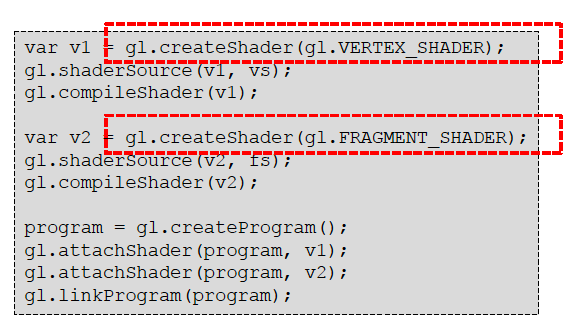
\includegraphics[width=.7\linewidth]{compile} 
\end{figure} 

\subsubsection{Workflow Recap}
\begin{figure}[H]
 \centering
 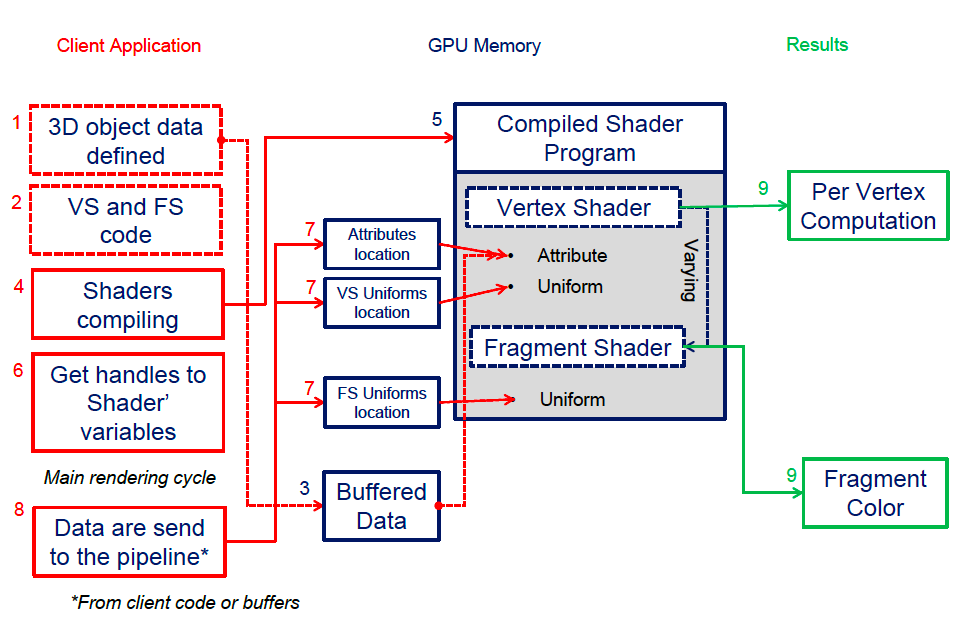
\includegraphics[width=.8\linewidth]{recap2} 
\end{figure} 

\subsection{Shader spaces}
The computation of light involves information about :
\begin{itemize}
\item normals
\item light position/direction
\item observer direction/position
\end{itemize}
The surface is defined by the direction of normals , if they are not computed in the same \textbf{space} as the \textbf{vertexes} the final light result is not going to be the one expected. When applying the \textbf{WVP Matrix} to the vertexes also normals should change otherwise this could happen :
\begin{figure}[H]
 \centering
 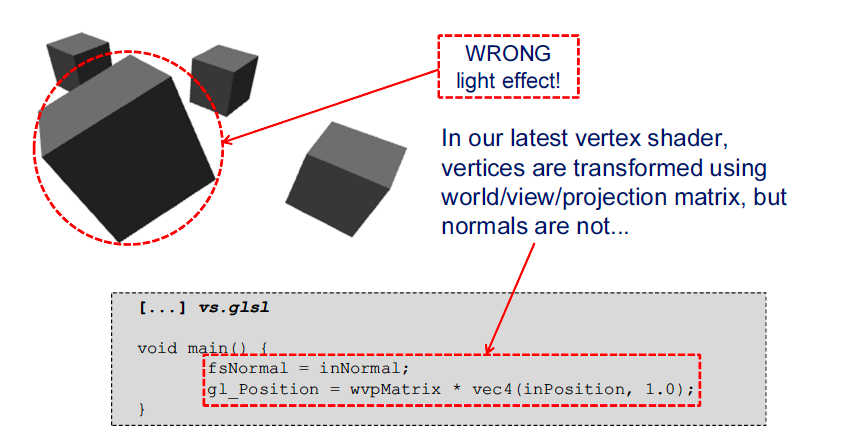
\includegraphics[width=.7\linewidth]{shaderspace} 
\end{figure} 
In order to achieve the intended light results, \textbf{data} about normals,lights and eye position must be expressed using the same coordinates system or \textbf{space}.
There are 4 main space systems:
\begin{itemize}
\item \textbf{World space}
\item \textbf{Camera space}
\item \textbf{Object space}
\item \textbf{Static space}
\end{itemize}

\subsubsection{World space}
When the illumination model is computed in \textbf{World Space} vertices positions and normals must be transformed according to the World Transforms. Is usually requires \textbf{three} matrices: 
\begin{itemize}
\item \textbf{WVP} projection ( as usual)
\item a matrix to transform \textbf{vertex positions}
\item a matrix to transform \textbf{normals} into worlds space
\end{itemize}
\begin{figure}[H]
 \centering
 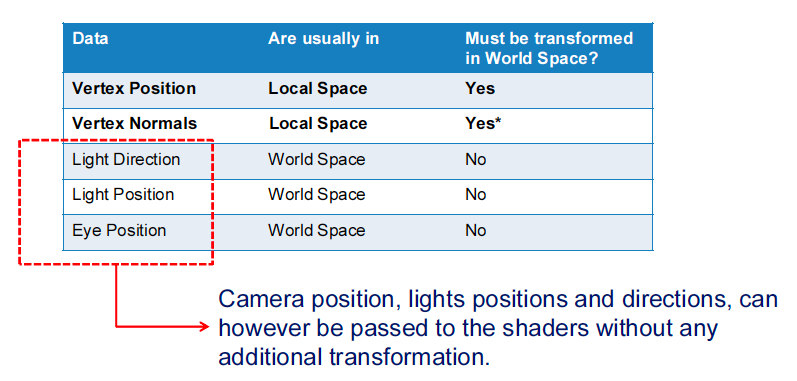
\includegraphics[width=.8\linewidth]{shaderspace2} 
\end{figure} 
To transform the \textbf{normal}  the \textbf{inverse} of the objects world matrix can be used if \textbf{no scalings}  are performed. Otherwise the \textbf{3x3 submatrix of the inverse transpose} should be used.
The world space light computation is\textbf{ computationally very expensive} as many vertex multiplication are performed.

\subsubsection{Camera space}
If the illumination in is computed in the \textbf{camera space} then position and normals must be transformed according to the \textbf{world transforms} and the \textbf{view transforms}. So this time \textbf{lights} (directions and positions)  must be transformed together with \textbf{objects and normals}.
\begin{figure}[H]
 \centering
 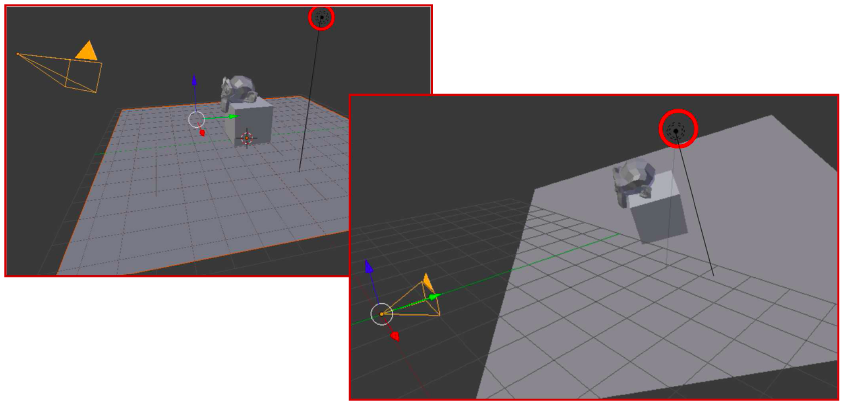
\includegraphics[width=.7\linewidth]{cameraspace} 
\end{figure} 
This requires passing \textbf{three} matrices to the VS to project \textbf{vertices},transform \textbf{positions} and transform \textbf{normals}.
For the light:
\begin{itemize}
\item The \textbf{light position} is transformed applying the \textbf{view transform}
\item The \textbf{light direction} is transformed applying the \textbf{inverse transpose} of the \textbf{3x3 submatrix} of the view transform (if \textbf{scaling} is used, otherwise just the 3x3 submatrix is fine).
\end{itemize} 
\begin{figure}[H]
 \centering
 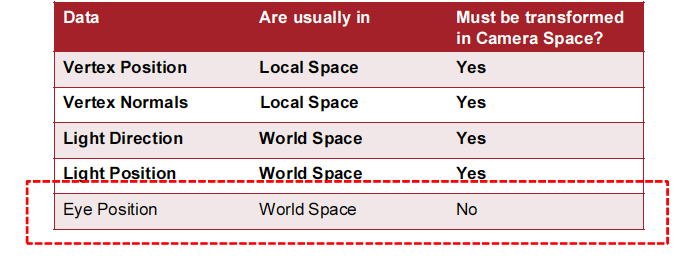
\includegraphics[width=.7\linewidth]{cameraspace2} 
\end{figure} 
The \textbf{observer direction} ( computed for specular Phong and Blinn models) can be obtained by \textbf{normalizing} the coordinates of the considered point of the object in the 3D space ( because after view transform the center of projection is now in the origin of the axis)

\subsubsection{Object space}
In object space the objects are the center of the world. This is useful as the \textbf{normals } and \textbf{vertex positions} do not to be changed. But the \textbf{light position and direction} along with the \textbf{observer} need to be transformed into the object \textbf{local coordinates}.
\begin{itemize}
\item for \textbf{light directions} the \textbf{inverse transpose 3x3 submatrix} of the \textbf{inverse World matrix} should be used.
\item for the \textbf{light positions} the \textbf{inverse of the World transform matrix} should be used.
\item to obtain the \textbf{observer direction} both \textbf{world} and \textbf{view} matrices should be inverted and applied to the origin ($(0,0,0,1)$) 
\end{itemize}
\begin{figure}[H]
 \centering
 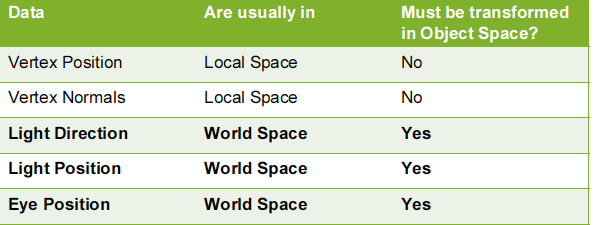
\includegraphics[width=.7\linewidth]{objectspace} 
\end{figure} 

\subsubsection{Static space}
In this space local and world coordinates are \textbf{identical} (world matrices are \textbf{identity} matrices).This also means that  world and object spaces are coincident. No transformation must be performed. It is the most simple to use but does not allow to \textbf{move objects during application}. This can be useful in medical or scientific visualization of fixed background in VR.

\subsubsection{Space recap}
\begin{figure}[H]
 \centering
 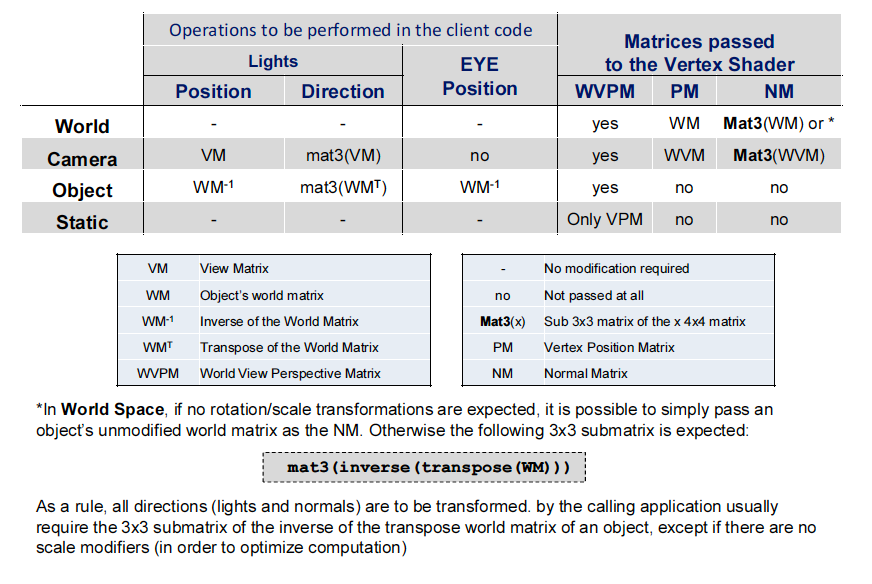
\includegraphics[width=.8\linewidth]{spacerecap} 
\end{figure} 

\subsection{GLSL Textures}
Textures are treated like any other data : declared in the client-code and handled sever-side. In the shaders \textbf{textures } can be handled using a \textbf{look-up function} $$ \texttt{vec4 texture2D(sampler2D sampler, vec2 coord)}$$
\begin{itemize}
\item \texttt{sampler2D sampler} is the identifier of texture object. It is passed from the \textbf{client code } to the \textbf{shader}.
\item \texttt{coord} are the \textbf{UV} coordinates for the lookup
\item \texttt{vect4} is the retuned object , a \textbf{color} in RGBa format.
\end{itemize}
Texels are extracted in the fragment shader using \texttt{sampler2D object} and \texttt{UV coordinates} by calling the \texttt{texture2D(texturefile,fsUVs)} which return a color (\texttt{vec4})
\begin{figure}[H]
 \centering
 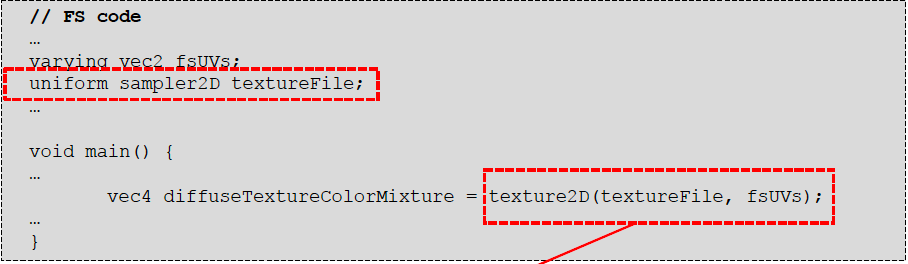
\includegraphics[width=.6\linewidth]{texture1} 
\end{figure} 
The \textbf{UV coordinates} can be associated to a vertex by including them into vertex formtat
\begin{figure}[H]
 \centering
 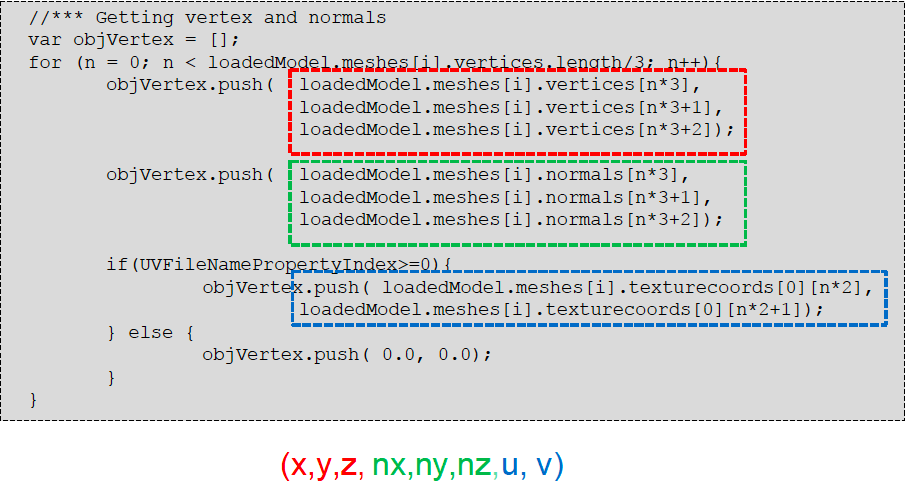
\includegraphics[width=.8\linewidth]{texture2} 
\end{figure} 

\subsubsection{Using texture : steps}
\begin{enumerate}
\item Allocate space on the GPU memory and its location stored in a variable
$$ \texttt{var texture = gl.createTexture()}$$
\item Specify which kind of texture will occupy that space and select it as the current one
$$ \texttt{gl.bindeTexture(gl.TEXTURE-2D,texture}$$
\item Load image to the texture object using HTML \texttt{Image()} to load an image file 
$$ \texttt{var image = new Image();}$$
This object has some properites :
\begin{itemize}
\item \texttt{image.src = imageURL} set or return URL
\item \texttt{image.onLoad = function() \{... \} }
\item \texttt{image.webglTexture} that returns the \textbf{texture object data}
\end{itemize}
\item Define more parameters to specify \textbf{texture attributes} in the callback function defined by \texttt{.onLoad}
\begin{figure}[H]
 \centering
 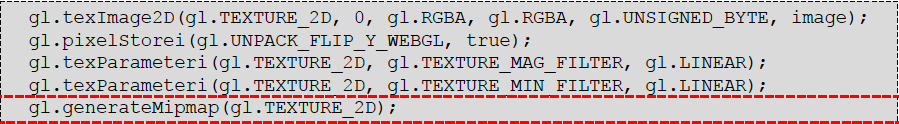
\includegraphics[width=.7\linewidth]{texture3} 
\end{figure} 
\begin{itemize}
\item The \texttt{texImage2D} that loads the image data into the texture object.
\item The \texttt{pixelStorei} set parameters for the pixels stored in the texture.It is used to \textbf{correct the orientation} of the image with respect to the UV-axis.
\item The \texttt{texParameteri} sets textures parameters for current texture unit. Here you can set properties for the \textbf{magnification}/\textbf{minification} filter using \texttt{gl.TEXTURE-MAG-FILTER}/\texttt{gl.TEXTURE-MIN-FILTER} . \\For \textbf{magnification} valid options are \texttt{gl.LINEAR,gl.NEAREST}\\
For \textbf{minification} valid options are \texttt{gl.LINEAR,gl.NEAREST,\\ gl.LINEAR-MIPMAP-LINEAR,...}
\item \texttt{generateMipmap} creates a set of textures for WebGLTexture object with image dimensions from the original size of the image down to a 1x1 image (used to create di MipMaps)
\end{itemize}
\end{enumerate}
During rendering:
\begin{figure}[H]
 \centering
 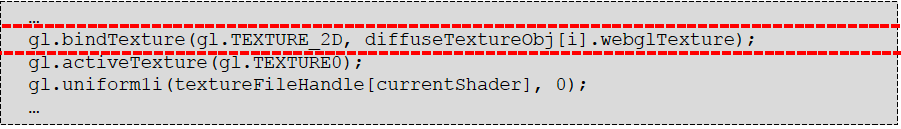
\includegraphics[width=.7\linewidth]{texture4} 
\end{figure} 
\begin{enumerate}
\item The texture must be selected again with \texttt{gl.BindTexture()}.The function uses the target specification of the texture and a reference to the texture object.
\item The binded texture is set as active unit and assigned to \textbf{level0}. Subsequent texture calls will affect only this unit.Depending on the specific implementation a different number of texture unit can be defined at one time and assigned to different levels (at least 8). More than 1 level is required if more than 1 texture is used on a face at once. Otherwise the same level can be used for different textures.
\item  Active texture is loaded at the $0^{th}$ level and the level is passed to the shader as uniform where it is received using $$ \texttt{uniform sampler2D textureFile }$$
\end{enumerate} 